% ============================================================
% Amazon-VT CFP 2026-2027 — 1-Page Abstract v3
% Proposal 2: Structured Validation Framework
% Primary: Agentic Evaluation / Secondary: Responsible AI
% ============================================================

\documentclass[10pt, letterpaper]{article}

% --- Packages ---
\usepackage[utf8]{inputenc}
\usepackage[T1]{fontenc}
\usepackage{lmodern}
\usepackage[margin=0.85in, top=0.75in, bottom=0.75in]{geometry}
\usepackage{hyperref}
\usepackage{natbib}
\usepackage{microtype}
\usepackage{parskip}
\setlength{\parskip}{0.25em}
\usepackage{enumitem}
\setlist{nosep, leftmargin=1.5em, topsep=0.2em}
\usepackage{graphicx}
\usepackage{caption}
\captionsetup{font=small, labelfont=bf, skip=3pt}
\usepackage{wrapfig}

\usepackage{titlesec}
\titlespacing*{\section}{0pt}{0.8em}{0.4em}

% --- Metadata ---
\title{\vspace{-2.5em}A Structured Validation Framework for\\Knowledge-Grounded and Multi-Agent AI Systems\vspace{-0.5em}}
\author{}
\date{}

% ============================================================
\begin{document}

\maketitle
\thispagestyle{empty}

\vspace{-2.5em}

\noindent\textbf{Primary Topic Area:} Foundation Model / Agentic Evaluation \hfill
\textbf{Secondary Topic Area:} Responsible Generative AI

\vspace{0.3em}

Knowledge-grounded and agentic AI systems are rapidly deployed in production settings, yet evaluation infrastructure has not kept pace. Standard benchmarks assess answer accuracy or safety robustness in isolation, but fail to measure the properties that determine reliability in compound AI systems: \textit{Is the retrieved evidence actually relevant? Does the cited source support the claim? Can the reasoning chain be traced and audited?} Recent work reveals that even retrieval-augmented generation (RAG) systems with valid-looking citations can produce references that do not fully support all statements~\cite{Ji2023HallucinationSurvey}, and that retrieval quality varies dramatically across query types, with naive top-$k$ retrieval degrading factuality when results are noisy or contradictory~\cite{Yan2024CRAG}. As systems move from single-model inference to multi-agent orchestration with heterogeneous retrieval~\cite{AWSBedrockHybridSearch2024,Edge2024GraphRAG}, the evaluation gap widens: there are no established benchmarks for measuring grounding integrity, provenance traceability, or coordination reliability across agent workflows.

\begin{wrapfigure}{r}{0.46\textwidth}
    \vspace{-0.8em}
    \centering
    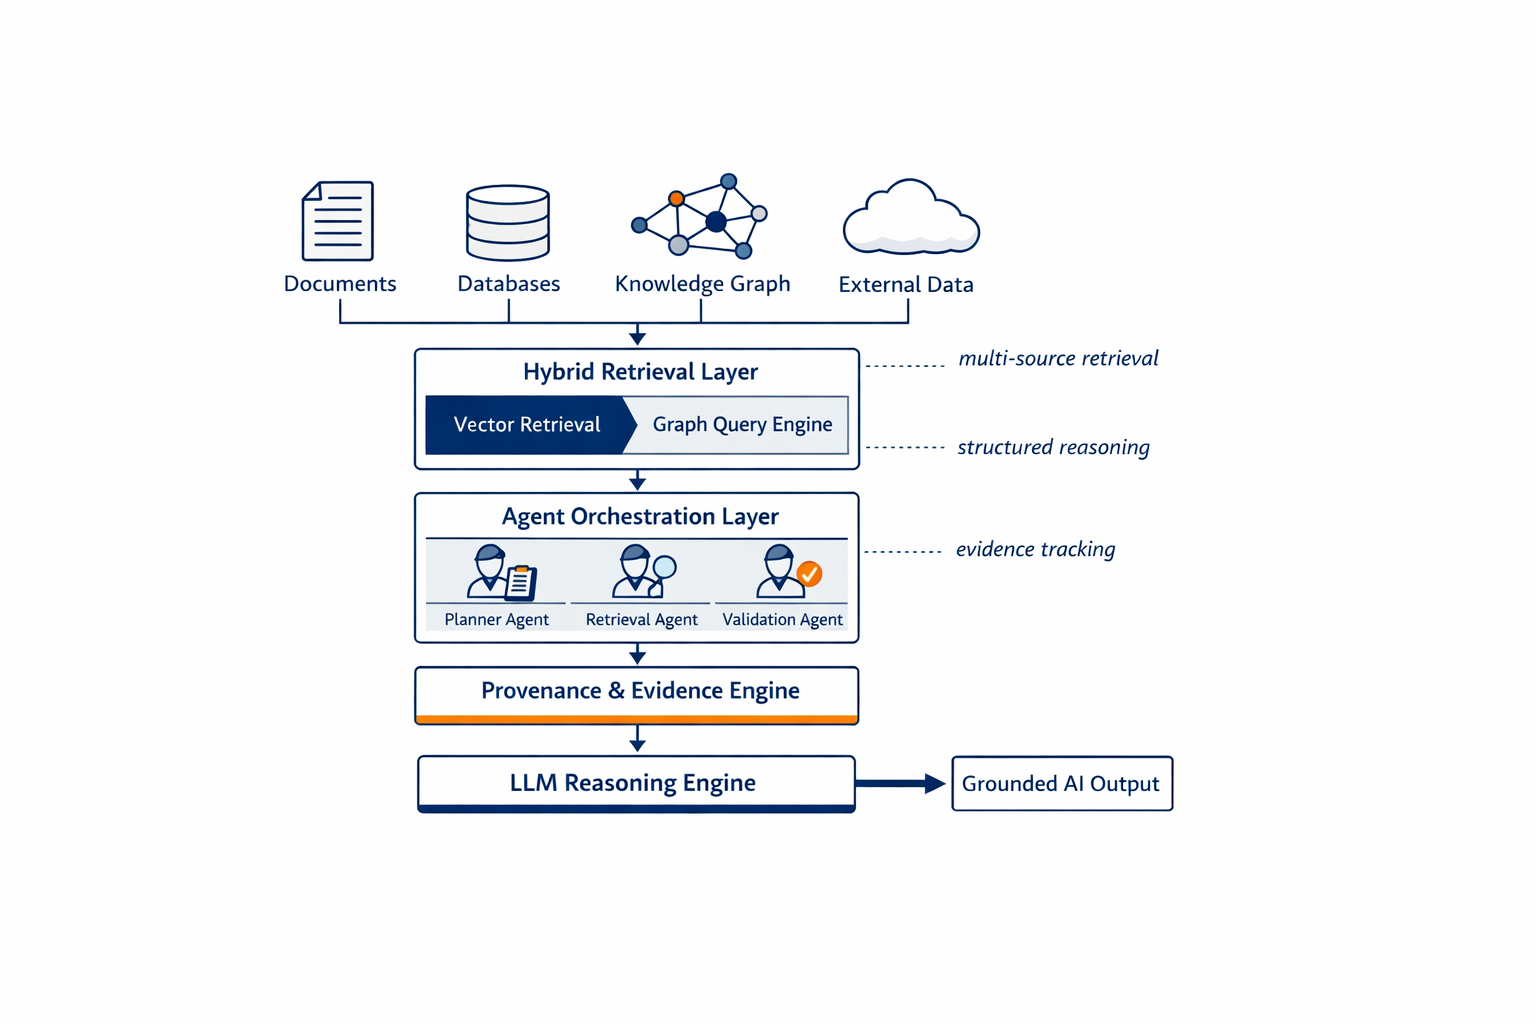
\includegraphics[width=0.44\textwidth]{images/architecture-diagram.png}
    \captionsetup{width=0.44\textwidth}
    \caption{\textbf{Validation Framework Architecture.} The framework evaluates knowledge-grounded agent systems across four dimensions: grounding integrity (retrieval relevance and evidence sufficiency), provenance traceability (span-level citation verification), reasoning robustness (performance under retrieval noise and contradictions), and coordination reliability (multi-agent failure modes and recovery). Evaluation signals align with emerging observability standards~\cite{OpenTelemetryGenAI2024}.}
    \label{fig:architecture}
    \vspace{-0.5em}
\end{wrapfigure}

This project proposes a \textbf{Structured Validation Framework (SVF)} that provides systematic evaluation infrastructure for knowledge-grounded and multi-agent AI systems. Unlike point-accuracy benchmarks, SVF evaluates along four complementary dimensions: (1)~\textbf{grounding integrity}---whether retrieved evidence is relevant, sufficient, and correctly attributed to claims; (2)~\textbf{provenance traceability}---whether reasoning chains can be audited from output back to specific source spans; (3)~\textbf{reasoning robustness}---whether systems degrade gracefully under retrieval noise, contradictory sources, and adversarial perturbations; and (4)~\textbf{coordination reliability}---whether multi-agent systems maintain consistency, recover from component failures, and avoid cascading errors. The framework embeds validation as a first-class component of agent execution pipelines, producing structured evaluation signals aligned with emerging observability standards~\cite{OpenTelemetryGenAI2024}.

This research investigates: (1)~what evaluation dimensions define reliable knowledge-grounded agent behavior beyond accuracy; (2)~how structured grounding mechanisms (knowledge graphs, hybrid retrieval) impact measurable robustness compared to vector-only RAG~\cite{Lewis2020RAG}; (3)~how validation loops can be embedded within agent orchestration to detect and recover from grounding failures in real time~\cite{Asai2024SelfRAG}; and (4)~how multi-agent coordination failures propagate and can be systematically benchmarked.

We will develop the SVF evaluation toolkit, benchmark tasks spanning scientific reasoning and enterprise decision-support, agent failure scenario simulations, and structured provenance scoring metrics. Experiments compare vector-only RAG, hybrid retrieval, and graph-augmented~\cite{Edge2024GraphRAG} agent systems across all four evaluation dimensions. Expected outcomes include the first structured evaluation framework for knowledge-grounded agentic AI, reproducible benchmark suites, and metrics for \textbf{grounding integrity, provenance traceability, and multi-agent reliability} that advance evaluation standards for responsible deployment of compound AI systems.

\newpage
\bibliographystyle{plainnat}
\bibliography{references}

\end{document}
